\section{Qualità di prodotto}
\label{sec:qdpr}
Per quantificare e valutare la qualità del prodotto software il gruppo \textit{SWEefty} ha deciso di attenersi allo standard ISO/IEC 25010, conosciuto anche come SQuaRE, che individua e definisce otto caratteristiche da considerare per costruire un prodotto software con un elevato livello di qualità. Ognuna di queste caratteristiche viene suddivisa in varie sottocaratteristiche(31 in totale), le quali, attraverso dei parametri misurabili  permettono una valutazione oggettiva del grado di conseguimento della caratteristica considerata.
 
	\subsection{Functional suitability}
	Con functional suitability si intende il livello di soddisfacimento dei bisogni espliciti o impliciti, raggiunto dal prodotto attraverso le sue funzionalità quando utilizzato sotto determinate condizioni.
		\subsubsection{Obiettivi}
			\begin{itemize}
				\item {\textbf{Functional completeness:} livello fino al quale l'insieme di funzioni copre tutti i compiti specificati e gli obiettivi dell'utente;}
				\item {\textbf{Functional correctness:} livello fino al quale un prodotto fornisce risultati corretti con il livello di precisione richiesto.}
			\end{itemize}
		\subsubsection{Metriche}
			\paragraph{Completezza dell'implementazione funzionale}\Spazio
			\begin{itemize}
				\item {\textbf{Range ottimale:} 100;}
				\item {\textbf{Range accettazione:} 100.}
			\end{itemize} 
            \subparagraph{Misurazioni}
            \begin{figure}[H]
            	\centering 
            	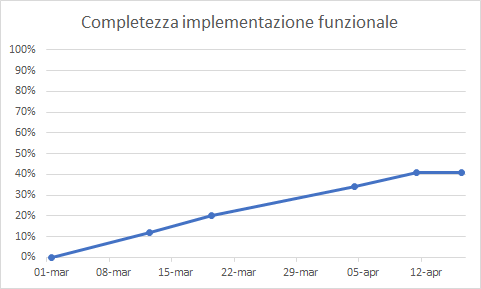
\includegraphics[width=0.7\textwidth]{Images/completezza-funzionale.png}
            	\caption{Serie storica della completezza dell'implementazione funzionale}
            	\label{cf} 
            \end{figure}
	\subsection{Reliability}
		Con reliability si intende il livello di performance mantenuto da specifiche funzioni di un prodotto in specifiche condizione per uno specifico periodo di tempo.
		\subsubsection{Obiettivi}
		\begin{itemize}
			\item {\textbf{Maturity:} livello fino al quale un prodotto garantisce Reliability durante un utilizzo normale;}
			\item {\textbf{Fault Tolerance:} livello fino al quale un prodotto riesce ad operare come previsto in presenza di fault di natura hardware o software.}
		\end{itemize}
		\subsubsection{Metriche}
			\paragraph{Densità di failure} \Spazio
			\begin{itemize}
				\item {\textbf{Range ottimale:} 0;}
				\item {\textbf{Range accettazione:} 0-10.}
			\end{itemize} 
			
	\subsection{Usability}
		Con usability si intende il livello a cui il prodotto può essere utilizzato da degli utenti specifici per raggiungere specifici obiettivi con efficacia, efficienza e soddisfazione in uno specifico contesto d'uso.  
		\subsubsection{Obiettivi}
		\begin{itemize}
			\item {\textbf{Appropriateness Recognizability:} livello a cui gli utenti riescono a riconoscere se il prodotto è adeguato per i loro bisogni;}
			\item {\textbf{Learnability:} livello di facilità con cui il prodotto può essere appreso dagli utenti per portare a termine determinati obiettivi con efficacia, efficienza, sicurezza e soddisfazione;} 
			\item {\textbf{User Interface Aesthetics:} livello a cui un interfaccia utente risulta piacevole per l'utente che la utilizza. }
			
		\end{itemize}
		\subsubsection{Metriche}
			\paragraph{Comprensibilità delle funzionalità offerte} \Spazio 
			\begin{itemize}
				\item {\textbf{Range ottimale:} 90-100;}
				\item {\textbf{Range accettazione:} 70-100.}
			\end{itemize} 
		   \subparagraph{Misurazioni}
		    \begin{figure}[H]
		   	\centering 
		    	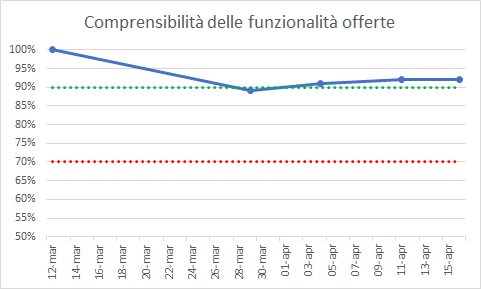
\includegraphics[width=0.7\textwidth]{Images/compr.png}
		    	\caption{Serie storica della Comprensibilità delle funzionalità offerte}
		    	\label{compr} 
		    \end{figure}
			\paragraph{Facilità di apprendimento} \Spazio 
			\begin{itemize}
				\item {\textbf{Range ottimale:} 0-10;}
				\item {\textbf{Range accettazione:} 0-20.}
			\end{itemize} 
			 \subparagraph{Misurazioni}
			\begin{figure}[H]
				\centering 
				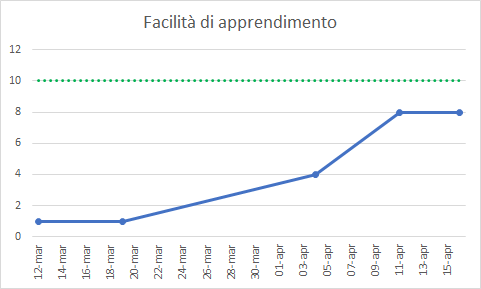
\includegraphics[width=0.7\textwidth]{Images/fac.png}
				\caption{Serie storica della facilità di apprendimento}
				\label{fac} 
			\end{figure}
	\subsection{Performance efficency}
		Con performance efficiency si intende il livello di performance relativo all'ammontare di risorse usate sotto determinate condizioni. 
		\subsubsection{Obiettivi}
			\begin{itemize}
				\item {\textbf{Time behaviour:} livello con cui il tempo di risposta e di processamento di un prodotto soddisfano certi requisiti durante l'esecuzione delle loro funzionalità;}
				\item {\textbf{Resource behaviour:} livello con cui la quantità e il tipo di risorse utilizzate da un prodotto durante l'esecuzione soddisfano certi requisiti.}
			\end{itemize}
		\subsubsection{Metriche}
			\paragraph{Tempo di risposta} \Spazio
			\begin{itemize}
				\item {\textbf{Range ottimale:} 0-3;}
				\item {\textbf{Range accettazione:} 0-8.}
			\end{itemize} 
		     \subparagraph{Misurazioni}
		      \begin{figure}[H]
		      \centering 
		      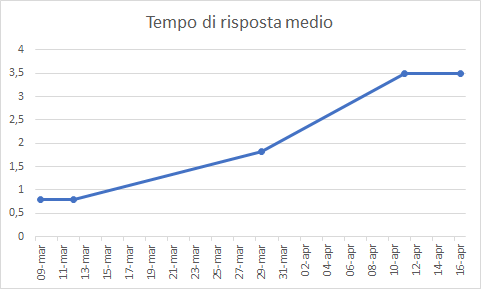
\includegraphics[width=0.7\textwidth]{Images/risposta.png}
		    	\caption{Serie storica del tempo di risposta medio}
		    	\label{risposta} 
		    \end{figure}
			
	\subsection{Maintainability}
		Con maintainability si intende il livello di efficacia e di efficienza con cui un prodotto può essere modificato dai manutentori incaricati.
		\subsubsection{Obiettivi}
		\begin{itemize}
			\item {\textbf{Analysability:} livello di efficacia ed efficienza con cui è possibile quantificare l'impatto di modifiche intenzionali. È anche la capacità di diagnosticare mancanze e cause di failures all'interno del prodotto; }
			\item{\textbf{Modifiability:} livello di efficacia ed efficienza con cui un prodotto può essere modificato senza introdurre difetti e degradare le qualità del prodotto già presenti;}
			\item{\textbf{Testability:} livello di efficacia ed efficienza con cui si possono essere creati dei test per valutare il prodotto.}
		\end{itemize}
		\subsubsection{Metriche}
			\paragraph{Capacità di analisi failure} \Spazio
			\begin{itemize}
				\item {\textbf{Range ottimale:} 80-100;}
				\item {\textbf{Range accettazione:} 60-100.}
			\end{itemize} 
			\paragraph{Impatto delle modifiche} \Spazio
			\begin{itemize}
				\item {\textbf{Range ottimale:} 0-10;}
				\item {\textbf{Range accettazione:} 0-20.}
			\end{itemize} 
		 \subparagraph{Misurazioni}
		\begin{figure}[H]
			\centering 
			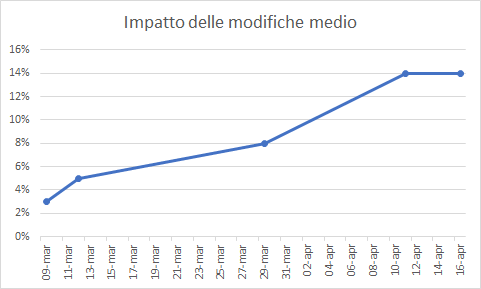
\includegraphics[width=0.7\textwidth]{Images/modifiche.png}
			\caption{Serie storica dell'impatto delle modifiche}
			\label{modifiche} 
		\end{figure}
